\documentclass[11pt,a4paper]{article}
\usepackage[utf8]{inputenc}
\usepackage[T1]{fontenc}
\usepackage{lmodern}
\usepackage[margin=1in]{geometry}
\usepackage{amsmath,amssymb,amsthm}
\usepackage{booktabs}
\usepackage{graphicx}
\usepackage{microtype}
\usepackage[numbers,sort&compress]{natbib}
\usepackage{xcolor}
\usepackage[colorlinks=true,linkcolor=blue!50!black,citecolor=blue!50!black,urlcolor=blue!50!black]{hyperref}
\usepackage{enumitem}
\usepackage{array}
\usepackage{caption}
\captionsetup{font=small,labelfont=bf}

\IfFileExists{numbers.tex}{% generated by experiments/make_numbers.py -- do not edit
\newcommand{\MetaSeed}{20260930}
\newcommand{\MetaSeedScaling}{20260931}
\newcommand{\MetaPython}{3.11.15}
\newcommand{\MetaNumpy}{2.4.6}
\newcommand{\MetaScipy}{1.17.1}
\newcommand{\MetaSklearn}{1.9.1}
\newcommand{\MetaSecondsValidation}{7}
\newcommand{\MetaSecondsFragility}{40}
\newcommand{\MetaSecondsScaling}{34}
\newcommand{\MetaSecondsTotal}{81}
\newcommand{\MetaMinutesTotal}{1.3}
\newcommand{\ExTwoMu}{\tfrac{7}{2}}
\newcommand{\ExTwoR}{3,4}
\newcommand{\ExTwoRp}{2,3,4}
\newcommand{\ExTwoTrials}{11}
\newcommand{\ExTwoSubsets}{26}
\newcommand{\ExTwoPairs}{3}
\newcommand{\ExTwoStabSel}{9/10}
\newcommand{\ExTwoDSupp}{1}
\newcommand{\ExTwoDBeta}{\hat\beta_{1}=\tfrac{3}{20}}
\newcommand{\ExTwoDC}{c_{2}=-\tfrac{1}{10}}
\newcommand{\ExTwoDCValTwo}{-\tfrac{1}{10}}
\newcommand{\ExTwoDMargOne}{5}
\newcommand{\ExTwoDMargTwo}{-1}
\newcommand{\ExTwoDRSupp}{2}
\newcommand{\ExTwoDRBeta}{\hat\beta_{2}=-\tfrac{5}{12}}
\newcommand{\ExTwoDRC}{c_{1}=\tfrac{11}{4}}
\newcommand{\ExTwoDRCValOne}{\tfrac{11}{4}}
\newcommand{\ExTwoDRMargOne}{4}
\newcommand{\ExTwoDRMargTwo}{-6}
\newcommand{\ExTwoDRpSupp}{1}
\newcommand{\ExTwoDRpBeta}{\hat\beta_{1}=\tfrac{1}{10}}
\newcommand{\ExTwoDRpC}{c_{2}=-\tfrac{17}{10}}
\newcommand{\ExTwoDRpCValTwo}{-\tfrac{17}{10}}
\newcommand{\ExTwoDRpMargOne}{4}
\newcommand{\ExTwoDRpMargTwo}{-2}
\newcommand{\ExTwoRows}{2 & -1 & 2 \\ 0 & 2 & -2 \\ 1 & 1 & 3 \\ 2 & -2 & -1 \\ -1 & 1 & 0}
\newcommand{\ExOneChecks}{12/12}
\newcommand{\ExOnebPresent}{yes}
\newcommand{\EoneSingleTests}{2760}
\newcommand{\EoneSingleAgree}{2760}
\newcommand{\EoneSinglePreserved}{2122}
\newcommand{\EoneSingleMaxDiff}{4\times 10^{-15}}
\newcommand{\EoneMultiTests}{7200}
\newcommand{\EoneMultiAgree}{7200}
\newcommand{\EoneMultiMaxDiff}{6\times 10^{-15}}
\newcommand{\EoneCdN}{104}
\newcommand{\EoneCdDis}{0}
\newcommand{\EoneCdMaxDiff}{2\times 10^{-13}}
\newcommand{\EoneReps}{15}
\newcommand{\EoneCorStable}{2114}
\newcommand{\EoneCorCertified}{1216}
\newcommand{\EoneCorCoverage}{58}
\newcommand{\EoneCorInstances}{120}
\newcommand{\EoneOracleUs}{1.1}
\newcommand{\EoneRefitUs}{442}
\newcommand{\EoneSpeedup}{399}
\newcommand{\EoneThroughputN}{14}
\newcommand{\EoneThroughputP}{6}
\newcommand{\EoneThroughputSubsets}{1001}
\newcommand{\EoneCorInstancesPerCell}{30}
\newcommand{\EtwoReps}{60}
\newcommand{\EtwoInstances}{480}
\newcommand{\EtwoKmax}{5}
\newcommand{\FamAp}{4}
\newcommand{\FamAb}{4}
\newcommand{\FamArho}{0.0}
\newcommand{\FamAc}{1.5}
\newcommand{\FamAs}{2}
\newcommand{\FamBp}{8}
\newcommand{\FamBb}{2}
\newcommand{\FamBrho}{0.5}
\newcommand{\FamBc}{1.0}
\newcommand{\FamBs}{2}
\newcommand{\EtwoANotFound}{0}
\newcommand{\EtwoAEmptySupport}{0}
\newcommand{\EtwoAFracOne}{52}
\newcommand{\EtwoAMax}{4}
\newcommand{\EtwoAMean}{1.73}
\newcommand{\EtwoATrueSupp}{78}
\newcommand{\EtwoASignedNeUnsigned}{0.0}
\newcommand{\EtwoASignedNeUnsignedCount}{0}
\newcommand{\EtwoAN}{240}
\newcommand{\EtwoATypesLeave}{51}
\newcommand{\EtwoATypesEnter}{43}
\newcommand{\EtwoATypesSwap}{6}
\newcommand{\EtwoATypesSign}{0}
\newcommand{\EtwoATypesN}{757}
\newcommand{\EtwoALeaveN}{240}
\newcommand{\EtwoALeaveNotFound}{12}
\newcommand{\EtwoALeaveMean}{2.4}
\newcommand{\EtwoAEnterN}{237}
\newcommand{\EtwoAEnterNotFound}{31}
\newcommand{\EtwoAEnterMean}{2.2}
\newcommand{\EtwoANGeTwo}{115}
\newcommand{\EtwoAKstarGeOne}{30}
\newcommand{\EtwoAKstarGap}{1.2}
\newcommand{\EtwoATimeAnyMs}{1}
\newcommand{\EtwoATimeLeaveMs}{22}
\newcommand{\EtwoATimeLeaveMaxS}{0.3}
\newcommand{\EtwoARefitsLeaveMax}{902}
\newcommand{\EtwoAOracleLeaveMax}{3472}
\newcommand{\EtwoBNotFound}{2}
\newcommand{\EtwoBEmptySupport}{8}
\newcommand{\EtwoBFracOne}{92}
\newcommand{\EtwoBMax}{3}
\newcommand{\EtwoBMean}{1.08}
\newcommand{\EtwoBTrueSupp}{21}
\newcommand{\EtwoBSignedNeUnsigned}{0.0}
\newcommand{\EtwoBSignedNeUnsignedCount}{0}
\newcommand{\EtwoBN}{240}
\newcommand{\EtwoBTypesLeave}{54}
\newcommand{\EtwoBTypesEnter}{25}
\newcommand{\EtwoBTypesSwap}{20}
\newcommand{\EtwoBTypesSign}{0}
\newcommand{\EtwoBTypesN}{1040}
\newcommand{\EtwoBLeaveN}{232}
\newcommand{\EtwoBLeaveNotFound}{0}
\newcommand{\EtwoBLeaveMean}{1.3}
\newcommand{\EtwoBEnterN}{240}
\newcommand{\EtwoBEnterNotFound}{31}
\newcommand{\EtwoBEnterMean}{1.5}
\newcommand{\EtwoBNGeTwo}{17}
\newcommand{\EtwoBKstarGeOne}{6}
\newcommand{\EtwoBKstarGap}{1.1}
\newcommand{\EtwoBTimeAnyMs}{2}
\newcommand{\EtwoBTimeLeaveMs}{6}
\newcommand{\EtwoBTimeLeaveMaxS}{0.3}
\newcommand{\EtwoBRefitsLeaveMax}{848}
\newcommand{\EtwoBOracleLeaveMax}{1470}
\newcommand{\EthreeCritExact}{90}
\newcommand{\EthreeCritCost}{10}
\newcommand{\EthreeMinCostAdjusted}{0.26}
\newcommand{\EthreeMinCostRaw}{0.46}
\newcommand{\EthreeAAnyOnestepExact}{97}
\newcommand{\EthreeAAnyOnestepExactSE}{1.2}
\newcommand{\EthreeAAnyOnestepExactNT}{93}
\newcommand{\EthreeAAnyOnestepCost}{1.34}
\newcommand{\EthreeAAnyOnestepCostAdj}{0.81}
\newcommand{\EthreeAAnyOnestepN}{240}
\newcommand{\EthreeAAnyAmipExact}{82}
\newcommand{\EthreeAAnyAmipExactSE}{2.5}
\newcommand{\EthreeAAnyAmipExactNT}{63}
\newcommand{\EthreeAAnyAmipCost}{1.28}
\newcommand{\EthreeAAnyAmipCostAdj}{0.77}
\newcommand{\EthreeAAnyAmipN}{240}
\newcommand{\EthreeAAnyCookExact}{66}
\newcommand{\EthreeAAnyCookExactSE}{3.1}
\newcommand{\EthreeAAnyCookExactNT}{57}
\newcommand{\EthreeAAnyCookCost}{1.23}
\newcommand{\EthreeAAnyCookCostAdj}{0.77}
\newcommand{\EthreeAAnyCookN}{240}
\newcommand{\EthreeALeaveOnestepExact}{95}
\newcommand{\EthreeALeaveOnestepExactSE}{1.4}
\newcommand{\EthreeALeaveOnestepExactNT}{93}
\newcommand{\EthreeALeaveOnestepCost}{0.48}
\newcommand{\EthreeALeaveOnestepCostAdj}{0.31}
\newcommand{\EthreeALeaveOnestepN}{228}
\newcommand{\EthreeALeaveAmipExact}{75}
\newcommand{\EthreeALeaveAmipExactSE}{2.9}
\newcommand{\EthreeALeaveAmipExactNT}{65}
\newcommand{\EthreeALeaveAmipCost}{0.46}
\newcommand{\EthreeALeaveAmipCostAdj}{0.31}
\newcommand{\EthreeALeaveAmipN}{228}
\newcommand{\EthreeALeaveCookExact}{67}
\newcommand{\EthreeALeaveCookExactSE}{3.1}
\newcommand{\EthreeALeaveCookExactNT}{66}
\newcommand{\EthreeALeaveCookCost}{0.49}
\newcommand{\EthreeALeaveCookCostAdj}{0.31}
\newcommand{\EthreeALeaveCookN}{228}
\newcommand{\EthreeAEnterOnestepExact}{86}
\newcommand{\EthreeAEnterOnestepExactSE}{2.4}
\newcommand{\EthreeAEnterOnestepExactNT}{78}
\newcommand{\EthreeAEnterOnestepCost}{0.76}
\newcommand{\EthreeAEnterOnestepCostAdj}{0.48}
\newcommand{\EthreeAEnterOnestepN}{206}
\newcommand{\EthreeAEnterAmipExact}{71}
\newcommand{\EthreeAEnterAmipExactSE}{3.1}
\newcommand{\EthreeAEnterAmipExactNT}{56}
\newcommand{\EthreeAEnterAmipCost}{0.72}
\newcommand{\EthreeAEnterAmipCostAdj}{0.45}
\newcommand{\EthreeAEnterAmipN}{206}
\newcommand{\EthreeAEnterCookExact}{27}
\newcommand{\EthreeAEnterCookExactSE}{3.1}
\newcommand{\EthreeAEnterCookExactNT}{11}
\newcommand{\EthreeAEnterCookCost}{1.04}
\newcommand{\EthreeAEnterCookCostAdj}{0.75}
\newcommand{\EthreeAEnterCookN}{206}
\newcommand{\EthreeBAnyOnestepExact}{100}
\newcommand{\EthreeBAnyOnestepExactSE}{0.0}
\newcommand{\EthreeBAnyOnestepExactNT}{100}
\newcommand{\EthreeBAnyOnestepCost}{0.73}
\newcommand{\EthreeBAnyOnestepCostAdj}{0.37}
\newcommand{\EthreeBAnyOnestepN}{238}
\newcommand{\EthreeBAnyAmipExact}{100}
\newcommand{\EthreeBAnyAmipExactSE}{0.4}
\newcommand{\EthreeBAnyAmipExactNT}{94}
\newcommand{\EthreeBAnyAmipCost}{0.77}
\newcommand{\EthreeBAnyAmipCostAdj}{0.40}
\newcommand{\EthreeBAnyAmipN}{238}
\newcommand{\EthreeBAnyCookExact}{87}
\newcommand{\EthreeBAnyCookExactSE}{2.2}
\newcommand{\EthreeBAnyCookExactNT}{76}
\newcommand{\EthreeBAnyCookCost}{0.62}
\newcommand{\EthreeBAnyCookCostAdj}{0.33}
\newcommand{\EthreeBAnyCookN}{238}
\newcommand{\EthreeBLeaveOnestepExact}{98}
\newcommand{\EthreeBLeaveOnestepExactSE}{0.9}
\newcommand{\EthreeBLeaveOnestepExactNT}{96}
\newcommand{\EthreeBLeaveOnestepCost}{0.58}
\newcommand{\EthreeBLeaveOnestepCostAdj}{0.29}
\newcommand{\EthreeBLeaveOnestepN}{232}
\newcommand{\EthreeBLeaveAmipExact}{95}
\newcommand{\EthreeBLeaveAmipExactSE}{1.5}
\newcommand{\EthreeBLeaveAmipExactNT}{79}
\newcommand{\EthreeBLeaveAmipCost}{0.56}
\newcommand{\EthreeBLeaveAmipCostAdj}{0.28}
\newcommand{\EthreeBLeaveAmipN}{232}
\newcommand{\EthreeBLeaveCookExact}{78}
\newcommand{\EthreeBLeaveCookExactSE}{2.7}
\newcommand{\EthreeBLeaveCookExactNT}{65}
\newcommand{\EthreeBLeaveCookCost}{0.53}
\newcommand{\EthreeBLeaveCookCostAdj}{0.29}
\newcommand{\EthreeBLeaveCookN}{232}
\newcommand{\EthreeBEnterOnestepExact}{88}
\newcommand{\EthreeBEnterOnestepExactSE}{2.3}
\newcommand{\EthreeBEnterOnestepExactNT}{80}
\newcommand{\EthreeBEnterOnestepCost}{0.52}
\newcommand{\EthreeBEnterOnestepCostAdj}{0.28}
\newcommand{\EthreeBEnterOnestepN}{209}
\newcommand{\EthreeBEnterAmipExact}{85}
\newcommand{\EthreeBEnterAmipExactSE}{2.5}
\newcommand{\EthreeBEnterAmipExactNT}{72}
\newcommand{\EthreeBEnterAmipCost}{0.49}
\newcommand{\EthreeBEnterAmipCostAdj}{0.26}
\newcommand{\EthreeBEnterAmipN}{209}
\newcommand{\EthreeBEnterCookExact}{23}
\newcommand{\EthreeBEnterCookExactSE}{2.9}
\newcommand{\EthreeBEnterCookExactNT}{1}
\newcommand{\EthreeBEnterCookCost}{0.78}
\newcommand{\EthreeBEnterCookCostAdj}{0.56}
\newcommand{\EthreeBEnterCookN}{209}
\newcommand{\EthreeAEnterOnestepShortfallSE}{1.7}
\newcommand{\EthreeBEnterOnestepShortfallSE}{1.1}
\newcommand{\EthreeNMin}{206}
\newcommand{\EthreeNMax}{240}
\newcommand{\EthreeSEMin}{0.4}
\newcommand{\EthreeSEMax}{3.1}
\newcommand{\EthreeAnyAdvantage}{none}
\newcommand{\EthreeNumAdvantage}{0}
\newcommand{\EthreeNumVerdicts}{18}
\newcommand{\EthreeAAnyKpredExact}{70}
\newcommand{\EthreeAAnyKpredUnder}{0}
\newcommand{\EthreeAAnyKpredOver}{30}
\newcommand{\EthreeALeaveKpredExact}{36}
\newcommand{\EthreeALeaveKpredUnder}{1}
\newcommand{\EthreeALeaveKpredOver}{63}
\newcommand{\EthreeAEnterKpredExact}{54}
\newcommand{\EthreeAEnterKpredUnder}{5}
\newcommand{\EthreeAEnterKpredOver}{41}
\newcommand{\EthreeBAnyKpredExact}{99}
\newcommand{\EthreeBAnyKpredUnder}{0}
\newcommand{\EthreeBAnyKpredOver}{1}
\newcommand{\EthreeBLeaveKpredExact}{84}
\newcommand{\EthreeBLeaveKpredUnder}{0}
\newcommand{\EthreeBLeaveKpredOver}{16}
\newcommand{\EthreeBEnterKpredExact}{80}
\newcommand{\EthreeBEnterKpredUnder}{11}
\newcommand{\EthreeBEnterKpredOver}{9}
\newcommand{\EthreeAOnestepMaxGap}{4}
\newcommand{\EthreeAOnestepMeanGap}{0.09}
\newcommand{\EthreeAAmipMaxGap}{8}
\newcommand{\EthreeAAmipMeanGap}{0.36}
\newcommand{\EthreeACookMaxGap}{6}
\newcommand{\EthreeACookMeanGap}{0.70}
\newcommand{\EthreeBOnestepMaxGap}{5}
\newcommand{\EthreeBOnestepMeanGap}{0.05}
\newcommand{\EthreeBAmipMaxGap}{5}
\newcommand{\EthreeBAmipMeanGap}{0.06}
\newcommand{\EthreeBCookMaxGap}{6}
\newcommand{\EthreeBCookMeanGap}{0.30}
\newcommand{\EfiveALeaveInstances}{228}
\newcommand{\EfiveALeaveFracInst}{51}
\newcommand{\EfiveALeaveFracPairs}{7.1}
\newcommand{\EfiveALeavePairs}{6960}
\newcommand{\EfiveAAnyInstances}{240}
\newcommand{\EfiveAAnyFracInst}{75}
\newcommand{\EfiveAAnyFracPairs}{14.9}
\newcommand{\EfiveAAnyPairs}{7029}
\newcommand{\EfiveBLeaveInstances}{232}
\newcommand{\EfiveBLeaveFracInst}{72}
\newcommand{\EfiveBLeaveFracPairs}{10.5}
\newcommand{\EfiveBLeavePairs}{8092}
\newcommand{\EfiveBAnyInstances}{238}
\newcommand{\EfiveBAnyFracInst}{72}
\newcommand{\EfiveBAnyFracPairs}{9.3}
\newcommand{\EfiveBAnyPairs}{10422}
\newcommand{\EfourKmax}{6}
\newcommand{\EfourNmaxExact}{34}
\newcommand{\EfourNmaxGreedy}{400}
\newcommand{\EfourATenMean}{1.43}
\newcommand{\EfourATenFracOne}{65}
\newcommand{\EfourATenNotFound}{0}
\newcommand{\EfourATenTime}{0.00}
\newcommand{\EfourATenOnestepExact}{98}
\newcommand{\EfourATenAmipExact}{95}
\newcommand{\EfourATenKpredExact}{85}
\newcommand{\EfourATenCostOnestep}{9.414}
\newcommand{\EfourATenInstances}{40}
\newcommand{\EfourAFourteenMean}{2.62}
\newcommand{\EfourAFourteenFracOne}{28}
\newcommand{\EfourAFourteenNotFound}{0}
\newcommand{\EfourAFourteenTime}{0.00}
\newcommand{\EfourAFourteenOnestepExact}{82}
\newcommand{\EfourAFourteenAmipExact}{68}
\newcommand{\EfourAFourteenKpredExact}{45}
\newcommand{\EfourAFourteenCostOnestep}{4.375}
\newcommand{\EfourAFourteenInstances}{40}
\newcommand{\EfourAEighteenMean}{2.35}
\newcommand{\EfourAEighteenFracOne}{28}
\newcommand{\EfourAEighteenNotFound}{0}
\newcommand{\EfourAEighteenTime}{0.00}
\newcommand{\EfourAEighteenOnestepExact}{92}
\newcommand{\EfourAEighteenAmipExact}{70}
\newcommand{\EfourAEighteenKpredExact}{48}
\newcommand{\EfourAEighteenCostOnestep}{5.462}
\newcommand{\EfourAEighteenInstances}{40}
\newcommand{\EfourATwentytwoMean}{3.38}
\newcommand{\EfourATwentytwoFracOne}{8}
\newcommand{\EfourATwentytwoNotFound}{1}
\newcommand{\EfourATwentytwoTime}{0.02}
\newcommand{\EfourATwentytwoOnestepExact}{77}
\newcommand{\EfourATwentytwoAmipExact}{59}
\newcommand{\EfourATwentytwoKpredExact}{46}
\newcommand{\EfourATwentytwoCostOnestep}{1.361}
\newcommand{\EfourATwentytwoInstances}{40}
\newcommand{\EfourATwentysixMean}{2.70}
\newcommand{\EfourATwentysixFracOne}{23}
\newcommand{\EfourATwentysixNotFound}{3}
\newcommand{\EfourATwentysixTime}{0.07}
\newcommand{\EfourATwentysixOnestepExact}{93}
\newcommand{\EfourATwentysixAmipExact}{78}
\newcommand{\EfourATwentysixKpredExact}{59}
\newcommand{\EfourATwentysixCostOnestep}{1.281}
\newcommand{\EfourATwentysixInstances}{30}
\newcommand{\EfourAThirtyMean}{3.50}
\newcommand{\EfourAThirtyFracOne}{3}
\newcommand{\EfourAThirtyNotFound}{2}
\newcommand{\EfourAThirtyTime}{0.20}
\newcommand{\EfourAThirtyOnestepExact}{82}
\newcommand{\EfourAThirtyAmipExact}{71}
\newcommand{\EfourAThirtyKpredExact}{54}
\newcommand{\EfourAThirtyCostOnestep}{0.678}
\newcommand{\EfourAThirtyInstances}{30}
\newcommand{\EfourAThirtyfourMean}{4.00}
\newcommand{\EfourAThirtyfourFracOne}{0}
\newcommand{\EfourAThirtyfourNotFound}{1}
\newcommand{\EfourAThirtyfourTime}{0.41}
\newcommand{\EfourAThirtyfourOnestepExact}{89}
\newcommand{\EfourAThirtyfourAmipExact}{68}
\newcommand{\EfourAThirtyfourKpredExact}{37}
\newcommand{\EfourAThirtyfourCostOnestep}{0.070}
\newcommand{\EfourAThirtyfourInstances}{20}
\newcommand{\EfourBTenMean}{1.00}
\newcommand{\EfourBTenFracOne}{100}
\newcommand{\EfourBTenNotFound}{0}
\newcommand{\EfourBTenTime}{0.00}
\newcommand{\EfourBTenOnestepExact}{100}
\newcommand{\EfourBTenAmipExact}{100}
\newcommand{\EfourBTenKpredExact}{100}
\newcommand{\EfourBTenCostOnestep}{10.355}
\newcommand{\EfourBTenInstances}{40}
\newcommand{\EfourBFourteenMean}{1.10}
\newcommand{\EfourBFourteenFracOne}{90}
\newcommand{\EfourBFourteenNotFound}{0}
\newcommand{\EfourBFourteenTime}{0.00}
\newcommand{\EfourBFourteenOnestepExact}{100}
\newcommand{\EfourBFourteenAmipExact}{100}
\newcommand{\EfourBFourteenKpredExact}{100}
\newcommand{\EfourBFourteenCostOnestep}{10.083}
\newcommand{\EfourBFourteenInstances}{40}
\newcommand{\EfourBEighteenMean}{1.12}
\newcommand{\EfourBEighteenFracOne}{88}
\newcommand{\EfourBEighteenNotFound}{0}
\newcommand{\EfourBEighteenTime}{0.00}
\newcommand{\EfourBEighteenOnestepExact}{100}
\newcommand{\EfourBEighteenAmipExact}{95}
\newcommand{\EfourBEighteenKpredExact}{95}
\newcommand{\EfourBEighteenCostOnestep}{10.161}
\newcommand{\EfourBEighteenInstances}{40}
\newcommand{\EfourBTwentytwoMean}{1.12}
\newcommand{\EfourBTwentytwoFracOne}{90}
\newcommand{\EfourBTwentytwoNotFound}{0}
\newcommand{\EfourBTwentytwoTime}{0.00}
\newcommand{\EfourBTwentytwoOnestepExact}{100}
\newcommand{\EfourBTwentytwoAmipExact}{98}
\newcommand{\EfourBTwentytwoKpredExact}{100}
\newcommand{\EfourBTwentytwoCostOnestep}{10.206}
\newcommand{\EfourBTwentytwoInstances}{40}
\newcommand{\EfourBTwentysixMean}{1.50}
\newcommand{\EfourBTwentysixFracOne}{67}
\newcommand{\EfourBTwentysixNotFound}{0}
\newcommand{\EfourBTwentysixTime}{0.00}
\newcommand{\EfourBTwentysixOnestepExact}{97}
\newcommand{\EfourBTwentysixAmipExact}{97}
\newcommand{\EfourBTwentysixKpredExact}{87}
\newcommand{\EfourBTwentysixCostOnestep}{8.694}
\newcommand{\EfourBTwentysixInstances}{30}
\newcommand{\EfourBThirtyMean}{1.40}
\newcommand{\EfourBThirtyFracOne}{67}
\newcommand{\EfourBThirtyNotFound}{0}
\newcommand{\EfourBThirtyTime}{0.00}
\newcommand{\EfourBThirtyOnestepExact}{100}
\newcommand{\EfourBThirtyAmipExact}{100}
\newcommand{\EfourBThirtyKpredExact}{97}
\newcommand{\EfourBThirtyCostOnestep}{8.762}
\newcommand{\EfourBThirtyInstances}{30}
\newcommand{\EfourBThirtyfourMean}{1.30}
\newcommand{\EfourBThirtyfourFracOne}{75}
\newcommand{\EfourBThirtyfourNotFound}{0}
\newcommand{\EfourBThirtyfourTime}{0.00}
\newcommand{\EfourBThirtyfourOnestepExact}{95}
\newcommand{\EfourBThirtyfourAmipExact}{100}
\newcommand{\EfourBThirtyfourKpredExact}{100}
\newcommand{\EfourBThirtyfourCostOnestep}{8.100}
\newcommand{\EfourBThirtyfourInstances}{20}
\newcommand{\EfourAFiftyMedian}{6}
\newcommand{\EfourAFiftyMeanOverN}{0.129}
\newcommand{\EfourAFiftyKstar}{1}
\newcommand{\EfourAFiftyBracket}{0.45}
\newcommand{\EfourAFiftyTimeMs}{5}
\newcommand{\EfourAHundredMedian}{6}
\newcommand{\EfourAHundredMeanOverN}{0.069}
\newcommand{\EfourAHundredKstar}{2}
\newcommand{\EfourAHundredBracket}{0.50}
\newcommand{\EfourAHundredTimeMs}{5}
\newcommand{\EfourATwohundredMedian}{10}
\newcommand{\EfourATwohundredMeanOverN}{0.049}
\newcommand{\EfourATwohundredKstar}{3}
\newcommand{\EfourATwohundredBracket}{0.49}
\newcommand{\EfourATwohundredTimeMs}{7}
\newcommand{\EfourAFourhundredMedian}{10}
\newcommand{\EfourAFourhundredMeanOverN}{0.028}
\newcommand{\EfourAFourhundredKstar}{5}
\newcommand{\EfourAFourhundredBracket}{0.57}
\newcommand{\EfourAFourhundredTimeMs}{10}
\newcommand{\EfourBFiftyMedian}{1}
\newcommand{\EfourBFiftyMeanOverN}{0.036}
\newcommand{\EfourBFiftyKstar}{0}
\newcommand{\EfourBFiftyBracket}{0.75}
\newcommand{\EfourBFiftyTimeMs}{2}
\newcommand{\EfourBHundredMedian}{2}
\newcommand{\EfourBHundredMeanOverN}{0.028}
\newcommand{\EfourBHundredKstar}{1}
\newcommand{\EfourBHundredBracket}{0.74}
\newcommand{\EfourBHundredTimeMs}{2}
\newcommand{\EfourBTwohundredMedian}{2}
\newcommand{\EfourBTwohundredMeanOverN}{0.012}
\newcommand{\EfourBTwohundredKstar}{0}
\newcommand{\EfourBTwohundredBracket}{0.82}
\newcommand{\EfourBTwohundredTimeMs}{2}
\newcommand{\EfourBFourhundredMedian}{4}
\newcommand{\EfourBFourhundredMeanOverN}{0.011}
\newcommand{\EfourBFourhundredKstar}{2}
\newcommand{\EfourBFourhundredBracket}{0.77}
\newcommand{\EfourBFourhundredTimeMs}{4}
\newcommand{\EfourAOnestepExactAll}{88}
\newcommand{\EfourAOnestepExactNT}{83}
\newcommand{\EfourAAmipExactNT}{64}
\newcommand{\EfourANT}{174}
\newcommand{\EfourANAll}{233}
\newcommand{\EfourAOnestepMaxGap}{6}
\newcommand{\EfourACostOnestepMedian}{3.65}
\newcommand{\EfourACostOnestepMedianBig}{0.774}
\newcommand{\EfourAOnestepExactBig}{84}
\newcommand{\EfourANBig}{113}
\newcommand{\EfourACostOnestepMedianBigAll}{0.68}
\newcommand{\EfourANBigAll}{120}
\newcommand{\EfourANotFoundAll}{7}
\newcommand{\EfourAKpredExactAll}{55}
\newcommand{\EfourBOnestepExactAll}{99}
\newcommand{\EfourBOnestepExactNT}{95}
\newcommand{\EfourBAmipExactNT}{89}
\newcommand{\EfourBNT}{38}
\newcommand{\EfourBNAll}{240}
\newcommand{\EfourBOnestepMaxGap}{1}
\newcommand{\EfourBCostOnestepMedian}{9.82}
\newcommand{\EfourBCostOnestepMedianBig}{9.343}
\newcommand{\EfourBOnestepExactBig}{98}
\newcommand{\EfourBNBig}{120}
\newcommand{\EfourBCostOnestepMedianBigAll}{9.34}
\newcommand{\EfourBNBigAll}{120}
\newcommand{\EfourBNotFoundAll}{0}
\newcommand{\EfourBKpredExactAll}{97}
}{}

\theoremstyle{plain}
\newtheorem{theorem}{Theorem}[section]
\newtheorem{proposition}[theorem]{Proposition}
\newtheorem{lemma}[theorem]{Lemma}
\newtheorem{corollary}[theorem]{Corollary}
\newtheorem{conjecture}[theorem]{Conjecture}
\theoremstyle{definition}
\newtheorem{definition}[theorem]{Definition}
\newtheorem{example}[theorem]{Example}
\theoremstyle{remark}
\newtheorem{remark}[theorem]{Remark}

\newcommand{\R}{\mathbb{R}}
\newcommand{\Q}{\mathbb{Q}}
\newcommand{\Sc}{S^{\mathrm{c}}}
\newcommand{\supp}{\operatorname{supp}}
\newcommand{\sgn}{\operatorname{sgn}}
\newcommand{\tr}{\operatorname{tr}}
\newcommand{\status}[1]{\textsf{\small [#1]}}
\newcommand{\Dm}{D\setminus R}
\newcommand{\Tk}{T_k}

\title{\textbf{Fragility of Lasso Variable Selection:}\\[2pt]
\large Removal Witnesses, Exact Deletion Tests, Non-Monotonicity and Computational Status}
\author{Luciano Silva Alarco\\
\small Pontificia Universidad Cat\'olica del Per\'u\\
\small ORCID 0000-0002-3395-3129}
\date{\small Working draft v0.1 --- research line TCD001 --- \today}

\begin{document}
\maketitle

\begin{abstract}
\noindent
We study how the set of variables selected by the Lasso changes when observations are removed from the data. For data $D=(X,y)$, a penalty $\mu$ and a rule that fixes the penalty on subsamples, a \emph{removal witness} for a target change (a given variable leaves the selected set, a given variable enters it, or the selected set changes at all) is a set $R$ of observations such that the Lasso on $D\setminus R$ exhibits the change; the \emph{fragility number} is the minimal $|R|$. Four things are established. (i)~An exact test, in closed form, of whether removing a set $R$ preserves the signed support: it follows from the KKT conditions and a Woodbury update, costs $O(|R|^3+p|R|)$ per set after an $O(nps)$ precomputation, and reduces for $|R|=1$ to a case-deletion formula of the Cook--Belsley type with the Lasso residual in place of the least-squares residual. It yields a cheap certificate that no single removal changes the support, and a polynomial-time (but loose) certificate for $k$ removals. (ii)~The witness family is not monotone: a variable can leave the support after removing $R$ and re-enter after removing a superset of $R$. We give a one-variable example that can be checked by hand and a two-variable example, verified in exact rational arithmetic, in which the exclusion is caused by a competing variable. (iii)~Deciding whether a deselection witness exists at all is NP-complete already for one predictor, by a direct reduction from \textsc{Subset Sum}; the selection direction is solvable in $O(n\log n)$ for one predictor; the hardness is weak (pseudo-polynomial algorithms exist) and nothing is proved for $p\ge2$. (iv)~On synthetic Gaussian designs with fixed seeds, exhaustive search made feasible by the exact test (up to $n=\EfourNmaxExact$, $|R|\le\EfourKmax$) gives exact fragility numbers: in a noisy regime the selected set changes after removing a single observation in \EtwoBFracOne\% of the instances with $n\le14$, in a strong-signal regime in \EtwoAFracOne\%; minimal witnesses are predominantly single events (one variable leaves or one enters) and one-element supersets of minimal witnesses restore the original support in a measurable fraction of cases. Three heuristics (one-step greedy by exact deletion effect, sorted scores in the style of the approximate maximum influence perturbation, Cook's distance) are compared with the exact minimum under a criterion fixed in advance; none meets it on these instances, mainly because exhaustive search with the closed-form test is itself cheap at these sizes. No novelty is claimed for the algebra; the contribution is to make the objects of the research line precise and to report what can and cannot be certified.
\end{abstract}

\section{Introduction}\label{sec:intro}

Variable selection with the Lasso~\citep{tibshirani1996} is known to be unstable: small changes of the data can change the selected set. This instability has been addressed statistically, by aggregating selections over random subsamples~\citep[stability selection,][]{meinshausen2010}, and asymptotically, by conditions under which the selected set is the true one with high probability~\citep{zhao2006,wainwright2009,buhlmann2011}. A different, finite-sample and combinatorial question is the subject of the research line to which this draft belongs (TCD001): \emph{how many observations must be removed, and which, for the selected set to change?} The question has a long history for the coefficients of least squares, where case-deletion diagnostics~\citep{cook1977,belsley1980} and the influence curve~\citep{hampel1974} measure the effect of dropping one observation, and where the worst-case effect of dropping a small fraction of the data has recently been studied under the name of approximate maximum influence perturbation~\citep{broderick2020} and through exact or certified algorithms for the sign of a regression coefficient~\citep{moitra2022,freund2023,kuschnig2021}. For a \emph{selection}, the quantity of interest is discrete, so the influence function does not apply directly, and the natural object is a set of observations, a \emph{witness}, together with its minimal size.

The public record of the line states that non-monotone changes and connections to known combinatorial problems were identified, and that novelty, computational advantage and some certificates were not sufficiently established. This draft gives the line a precise core and settles, in the negative where that is the honest answer, the three points that were left open.

\begin{enumerate}[leftmargin=2em]
\item \textbf{Definitions} (Section~\ref{sec:setting}): penalty rules on subsamples, removal witnesses, fragility numbers, monotonicity.
\item \textbf{Exact deletion test and certificates} (Section~\ref{sec:exact}): a closed-form test of whether removing a set of observations preserves the signed support (Proposition~\ref{prop:exact}); its single-removal form, which is a Cook--Belsley deletion formula with the Lasso residual (Corollary~\ref{cor:single}); and a polynomial-time certificate that no $k$ removals change the support (Proposition~\ref{prop:cert}). All are proved and verified numerically against refits.
\item \textbf{Non-monotonicity} (Section~\ref{sec:nonmono}): the witness family is not closed under supersets; a hand-checkable example with $p=1$ and an exactly verified example with $p=2$ in which the mechanism is competition between variables.
\item \textbf{Computational status} (Section~\ref{sec:hardness}): existence of a deselection witness is NP-complete for $p=1$ by a reduction from \textsc{Subset Sum}; selection witnesses for $p=1$ are easy; the general case is open and stated as such.
\item \textbf{Experiments} (Section~\ref{sec:experiments}): exact fragility numbers by exhaustive search, the distribution of witness types, the frequency of non-monotone pairs, scaling with $n$, and a comparison of three heuristics with the exact minimum under a criterion fixed before the run.
\end{enumerate}

\paragraph{Scope.} The paper is methodological. It makes no claim about any real data set, and it does not propose the fragility number as a replacement for stability selection or for asymptotic theory; Remark~\ref{rem:stabsel} states the one implication between the two that follows from the definitions. Every number in the text is produced by the scripts of Appendix~\ref{app:repro} with fixed seeds. Section~\ref{sec:claims} lists all claims with their status: proved here, classical, from the literature, computationally verified, or conjectural.

\section{Setting and definitions}\label{sec:setting}

Let $D=(X,y)$ with $X\in\R^{n\times p}$, $y\in\R^n$, no intercept and columns as given. For $\mu>0$ the Lasso objective in sum form is
\begin{equation}\label{eq:lasso}
L_D(\beta;\mu)=\tfrac12\lVert y-X\beta\rVert_2^2+\mu\lVert\beta\rVert_1 ,
\end{equation}
which is the objective of scikit-learn's \texttt{Lasso} with \texttt{alpha}$=\mu/n$~\citep{pedregosa2011}. We write $\hat\beta(D;\mu)$ for its minimiser when it is unique, $S(D)=\supp\hat\beta$ for the \emph{support} (the selected set) and $(S,s)$ with $s=\sgn\hat\beta_S\in\{\pm1\}^S$ for the \emph{signed support}. Two facts from~\citet{tibshirani2013} are used throughout: if the columns of $X$ are in general position the minimiser is unique for every $y$ and $\mu>0$; and if the \emph{equicorrelation set} $E=\{j:\lvert X_j^{\top}(y-X\hat\beta)\rvert=\mu\}$ has $X_E$ of full column rank, the minimiser is unique and is determined by the linear system of the KKT conditions on $E$. Conversely a unique minimiser has $X_S$ of full column rank (Lemma~\ref{lem:rank}). \status{literature}

\begin{definition}[Penalty rule]\label{def:rule}
A \emph{penalty rule} assigns to the subsample $\Dm$ of size $n-k$ a penalty $\mu_k$. Two rules are used: the \emph{constant rule} (C), $\mu_k=\mu$, and the \emph{proportional rule} (P), $\mu_k=\mu(n-k)/n$, which keeps scikit-learn's \texttt{alpha} fixed and is what a practitioner does who refits ``with the same $\lambda$'' in the mean-squared-error parametrisation.
\end{definition}

\begin{definition}[Removal witness, fragility number]\label{def:witness}
Fix $D$, $\mu$, a rule, and let $(S,s)$ be the signed support on $D$. A \emph{target} $\Pi$ is a property of the signed support of the Lasso on a subsample, relative to $(S,s)$; the targets used here are
\begin{itemize}[leftmargin=2em,itemsep=1pt]
\item \textsc{any}: $S(\Dm)\neq S$ (unsigned), or $(S(\Dm),s(\Dm))\neq(S,s)$ (signed);
\item \textsc{leave}$(j)$, $j\in S$: $j\notin S(\Dm)$;
\item \textsc{enter}$(j)$, $j\notin S$: $j\in S(\Dm)$.
\end{itemize}
A \emph{removal witness} for $\Pi$ is a proper subset $R\subsetneq[n]$ such that the Lasso on $\Dm$ with penalty $\mu_{|R|}$ has a unique minimiser and $\Pi$ holds. The \emph{witness family} is $W_\Pi(D)=\{R:\ R\text{ is a witness}\}$ and the \emph{fragility number} is $f_\Pi(D)=\min\{|R|:R\in W_\Pi(D)\}$, with $f_\Pi(D)=\infty$ if $W_\Pi(D)=\emptyset$.
\end{definition}

The signed and unsigned versions of \textsc{any} differ only when a coefficient changes sign without leaving the support; $f_{\textsc{any}}^{\mathrm{signed}}\le f_{\textsc{any}}$ and the experiments report how often the two differ. Witnesses for the signed target are decided without refitting by Proposition~\ref{prop:exact}.

\begin{definition}[Monotonicity]\label{def:mono}
The target $\Pi$ is \emph{monotone on $D$} if $R\in W_\Pi(D)$ and $R\subseteq R'\subsetneq[n]$ imply $R'\in W_\Pi(D)$. A \emph{non-monotone pair} is a pair $R\subsetneq R'$ with $R\in W_\Pi(D)$ and $R'\notin W_\Pi(D)$; for \textsc{leave}$(j)$ this means that $j$ leaves the support after removing $R$ and re-enters after removing $R'$.
\end{definition}

\begin{lemma}\label{lem:rank}
If the minimiser of \eqref{eq:lasso} is unique with support $S$, then $X_S$ has full column rank.
\end{lemma}
\begin{proof}
If $X_S\eta=0$ with $\eta\neq0$, extend $\eta$ by zeros. For $|t|$ small, $\hat\beta+t\eta$ has the same fit and the same signs on $S$, so $L_D(\hat\beta+t\eta)=L_D(\hat\beta)+t\mu\,s^{\top}\eta$. If $s^{\top}\eta\ne0$ one sign of $t$ decreases the objective, contradicting optimality; if $s^{\top}\eta=0$ every such $\hat\beta+t\eta$ is a minimiser, contradicting uniqueness. (This is part of the characterisation in~\citealp{tibshirani2013}.)
\end{proof}

\section{An exact deletion test and two certificates}\label{sec:exact}

Throughout this section $\hat\beta$ is the unique minimiser on $D$ with signed support $(S,s)$, $|S|=s_0\ge0$ (we write $s_0$ for the size to avoid a clash with the sign vector), $X_S$ has full column rank, and
\[
A=X_S^{\top}X_S,\quad r=y-X\hat\beta,\quad c=X^{\top}r,\quad V=X_SA^{-1}\ (\text{rows }v_i^{\top}),\quad h_i=x_{iS}^{\top}A^{-1}x_{iS},\quad \tilde X=(I-X_SA^{-1}X_S^{\top})X_{\Sc},
\]
so that $c_S=\mu s$, $|c_j|\le\mu$ for $j\notin S$, $h_i\in[0,1]$ are the leverages of the active-set regression and $\tilde X_j$ is the residual of $X_j$ regressed on $X_S$. For $R\subseteq[n]$ with $|R|=k$ let $U=X_{R,S}\in\R^{k\times s_0}$ and $H_R=UA^{-1}U^{\top}$, the $R\times R$ block of the projection $X_SA^{-1}X_S^{\top}$.

\begin{proposition}[Exact removal test]\label{prop:exact}\status{proved here}
Let $R\subsetneq[n]$, $|R|=k$, and let $\mu'$ be the penalty on $\Dm$, $\delta=\mu-\mu'$.
\begin{enumerate}[label=(\alph*),leftmargin=2em]
\item If $I-H_R$ is singular, $(S,s)$ is not the signed support of a unique minimiser on $\Dm$.
\item If $I-H_R$ is nonsingular, put $e_R=(I-H_R)^{-1}r_R$, $w=A^{-1}s$, $z=w+V_R^{\top}(I-H_R)^{-1}Uw$, and
\begin{align}
\tilde\beta_S&=\hat\beta_S-V_R^{\top}e_R+\delta z,\label{eq:betatilde}\\
\tilde c_j&=c_j-\tilde X_{R,j}^{\top}e_R-\delta\,\bigl(X_j^{\top}X_S-X_{R,j}^{\top}U\bigr)z,\qquad j\notin S.\label{eq:ctilde}
\end{align}
Then $(S,s)$ is the signed support of a minimiser on $\Dm$ if and only if $s_j\tilde\beta_j>0$ for all $j\in S$ and $|\tilde c_j|\le\mu'$ for all $j\notin S$. If moreover $|\tilde c_j|<\mu'$ for all $j\notin S$, the minimiser on $\Dm$ is unique and equals $\tilde\beta$ (extended by zeros).
\end{enumerate}
Under the constant rule $\delta=0$ and the last terms of \eqref{eq:betatilde}--\eqref{eq:ctilde} vanish.
\end{proposition}

\begin{proof}
A vector $\beta$ with signed support $(S,s)$ minimises the objective on $\Dm$ if and only if it satisfies the KKT conditions
\begin{equation}\label{eq:kkt}
X_{S,-R}^{\top}\bigl(y_{-R}-X_{S,-R}\beta_S\bigr)=\mu's,\qquad \bigl|X_{j,-R}^{\top}(y_{-R}-X_{S,-R}\beta_S)\bigr|\le\mu'\ (j\notin S),\qquad s_j\beta_j>0\ (j\in S).
\end{equation}
The matrix of the linear system is $A'=X_{S,-R}^{\top}X_{S,-R}=A-U^{\top}U$, and by the matrix determinant lemma $\det A'=\det A\cdot\det(I-UA^{-1}U^{\top})=\det A\cdot\det(I-H_R)$.

(a) If $I-H_R$ is singular then $X_{S,-R}$ is rank deficient, and by Lemma~\ref{lem:rank} no unique minimiser on $\Dm$ has support $S$.

(b) If $I-H_R$ is nonsingular, the Woodbury identity~\citep{sherman1950,hager1989} gives $A'^{-1}=A^{-1}+A^{-1}U^{\top}(I-H_R)^{-1}UA^{-1}$, and the unique solution of the linear system is $\beta_S=A'^{-1}(X_S^{\top}y-U^{\top}y_R-\mu's)$. Write $X_S^{\top}y-\mu s=A\hat\beta_S$ (the KKT equation on $D$) so that $X_S^{\top}y-U^{\top}y_R-\mu' s=A\hat\beta_S-U^{\top}y_R+\delta s$. Then
\[
A'^{-1}(A\hat\beta_S-U^{\top}y_R)=\hat\beta_S+A^{-1}U^{\top}\bigl[(I-H_R)^{-1}U\hat\beta_S-y_R-(I-H_R)^{-1}H_Ry_R\bigr]=\hat\beta_S-A^{-1}U^{\top}(I-H_R)^{-1}\bigl(y_R-U\hat\beta_S\bigr),
\]
using $y_R+(I-H_R)^{-1}H_Ry_R=(I-H_R)^{-1}y_R$; since $y_R-U\hat\beta_S=r_R$ and $A^{-1}U^{\top}=V_R^{\top}$, this is $\hat\beta_S-V_R^{\top}e_R$. The remaining term $\delta A'^{-1}s=\delta z$ by the same identity, which proves \eqref{eq:betatilde}. For $j\notin S$, with $\beta_S=\hat\beta_S-V_R^{\top}e_R$ the full-length residual is $\tilde r=r+X_SV_R^{\top}e_R$, whose $R$-block is $r_R+H_Re_R=(I-H_R)^{-1}r_R=e_R$; hence
\[
X_{j,-R}^{\top}\tilde r_{-R}=X_j^{\top}\tilde r-X_{R,j}^{\top}e_R=c_j+X_j^{\top}X_SA^{-1}U^{\top}e_R-X_{R,j}^{\top}e_R=c_j-\bigl(X_{R,j}-UA^{-1}X_S^{\top}X_j\bigr)^{\top}e_R=c_j-\tilde X_{R,j}^{\top}e_R ,
\]
and the additional coefficient $\delta z$ contributes $-\delta X_{j,-R}^{\top}X_{S,-R}z=-\delta(X_j^{\top}X_S-X_{R,j}^{\top}U)z$, which proves \eqref{eq:ctilde}. The equivalence is now \eqref{eq:kkt}. If the inactive inequalities are strict, the equicorrelation set on $\Dm$ is $S$ and $X_{S,-R}$ has full column rank, so the minimiser is unique~\citep{tibshirani2013}.
\end{proof}

The test costs $O(k^3+pk)$ per set $R$ after the $O(nps_0+s_0^3)$ precomputation of $V$, $h$, $\tilde X$ and $c$; it is vectorised over all subsets of a given size in the code, and Section~\ref{sec:experiments} measures its throughput against refits. Boundary cases ($s_j\tilde\beta_j=0$ or $|\tilde c_j|=\mu'$) have probability zero for continuous designs and are counted, not hidden, in the validation.

\begin{corollary}[Single removal; a stability margin]\label{cor:single}\status{proved here}
Under the constant rule, for $R=\{i\}$ one has $h_i<1$, $e_i=r_i/(1-h_i)$,
\[
\tilde\beta_S=\hat\beta_S-v_i\,e_i,\qquad \tilde c_j=c_j-\tilde x_{ij}\,e_i\quad(j\notin S),
\]
so removing observation $i$ preserves $(S,s)$ if and only if $s_j(\hat\beta_j-v_{ij}e_i)>0$ for $j\in S$ and $|c_j-\tilde x_{ij}e_i|<\mu$ for $j\notin S$ (boundary cases aside). In particular, with $m=\min_{j\in S}|\hat\beta_j|$ and $\gamma=\min_{j\notin S}(\mu-|c_j|)$, the \emph{instability index}
\[
\iota_i=|e_i|\max\Bigl\{\frac{\lVert v_i\rVert_\infty}{m},\ \frac{\max_{j\notin S}|\tilde x_{ij}|}{\gamma}\Bigr\}
\]
satisfies: $\iota_i<1$ implies that removing $i$ preserves $(S,s)$, and $\max_i\iota_i<1$ implies $f^{\mathrm{signed}}_{\textsc{any}}(D)\ge2$. Both statements are checkable in $O(np)$ time after the precomputation.
\end{corollary}
\begin{proof}
Specialise Proposition~\ref{prop:exact} to $k=1$: $H_R=h_i$, $I-H_R$ is nonsingular because $h_i<1$ when $X_{S,-i}$ has full column rank (and $h_i=1$ is excluded by part (a) only in the rank-deficient case, which the code treats as a change). The sufficient condition is the triangle inequality applied to \eqref{eq:betatilde}--\eqref{eq:ctilde}.
\end{proof}

\begin{remark}[Relation to case-deletion diagnostics]\label{rem:cook}
$v_ie_i=A^{-1}x_{iS}\,r_i/(1-h_i)$ is the DFBETA formula of~\citet{belsley1980} for the regression of $y$ on $X_S$, with the Lasso residual $r_i$ in place of the least-squares residual, and $e_i$ is the corresponding leave-one-out residual; $\tilde c_j-c_j=-\tilde x_{ij}e_i$ has no least-squares counterpart and is what decides entries. Cook's distance~\citep{cook1977} of the active-set regression is proportional to $h_ie_i^2$ and is used below as a target-agnostic heuristic. \status{classical}
\end{remark}

\begin{proposition}[Polynomial certificate for $k$ removals, constant rule]\label{prop:cert}\status{proved here}
For a vector $a\ge0$ let $\Tk(a)$ be the sum of its $k$ largest entries. Suppose $\Tk(h)<1$. Then for every $R$ with $|R|\le k$ the matrix $I-H_R$ is nonsingular and, with $\tilde\beta$ as in \eqref{eq:betatilde} and $\delta=0$,
\begin{align*}
|\tilde\beta_j-\hat\beta_j|&\le B_j(k):=\Tk\bigl(|v_{\cdot j}|\odot|r|\bigr)+\sqrt{\Tk(v_{\cdot j}^2)\,\Tk(r^2)}\;\frac{\Tk(h)}{1-\Tk(h)}\qquad(j\in S),\\
|\tilde c_j-c_j|&\le C_j(k):=\Tk\bigl(|\tilde x_{\cdot j}|\odot|r|\bigr)+\sqrt{\Tk(\tilde x_{\cdot j}^2)\,\Tk(r^2)}\;\frac{\Tk(h)}{1-\Tk(h)}\qquad(j\notin S).
\end{align*}
Consequently, if $B_j(k)<|\hat\beta_j|$ for all $j\in S$ and $C_j(k)<\mu-|c_j|$ for all $j\notin S$, then no removal of at most $k$ observations changes the signed support: $f^{\mathrm{signed}}_{\textsc{any}}(D)\ge k+1$. The certificate costs $O(nps_0+n\log n)$ and is monotone in $k$; we write $k^\ast(D)$ for the largest certified $k$ ($k^\ast=0$ if none).
\end{proposition}
\begin{proof}
$H_R$ is a principal submatrix of a projection, so $0\preceq H_R\preceq I$ and $\lambda_{\max}(H_R)\le\tr H_R=\sum_{i\in R}h_i\le\Tk(h)<1$; hence $I-H_R$ is nonsingular with $\lVert(I-H_R)^{-1}\rVert_2\le(1-\Tk(h))^{-1}$ and $\lVert e_R\rVert_2\le\lVert r_R\rVert_2/(1-\Tk(h))\le\sqrt{\Tk(r^2)}/(1-\Tk(h))$. From $(I-H_R)e_R=r_R$ we have $e_R=r_R+H_Re_R$, so
\[
\tilde\beta_j-\hat\beta_j=-v_{R,j}^{\top}e_R=-\sum_{i\in R}v_{ij}r_i-v_{R,j}^{\top}H_Re_R ,
\]
whose first term is bounded by $\Tk(|v_{\cdot j}|\odot|r|)$ and whose second is bounded by $\lVert v_{R,j}\rVert_2\lVert H_R\rVert_2\lVert e_R\rVert_2\le\sqrt{\Tk(v^2_{\cdot j})}\,\Tk(h)\sqrt{\Tk(r^2)}/(1-\Tk(h))$. The bound for $\tilde c_j$ is identical with $\tilde x_{\cdot j}$ in place of $v_{\cdot j}$. Under the hypotheses, every $R$ with $|R|\le k$ satisfies the conditions of Proposition~\ref{prop:exact}(b) strictly, so the signed support is preserved.
\end{proof}

The first term of $B_j(k)$ is the additive, ``sum of single-deletion effects'' approximation on which sorted-influence heuristics rest~\citep{broderick2020}; the second term controls the interaction between removed observations. Since $\sum_ih_i=s_0$, the hypothesis $\Tk(h)<1$ restricts the certificate to $k<n/s_0$ roughly, and the experiments show that it is loose: it certifies $k^\ast\ge1$ in only a fraction of the instances whose true fragility number is at least $2$ (Table~\ref{tab:e1b}).

\begin{remark}[Stability selection]\label{rem:stabsel}\status{proved here}
Stability selection~\citep{meinshausen2010} refits on subsamples of size $\lfloor n/2\rfloor$ with the same per-observation penalty (rule P) and reports the selection frequency $\Pi_j$ of variable $j$. A subsample of size $\lfloor n/2\rfloor$ is $\Dm$ with $|R|=\lceil n/2\rceil$, so $f_{\textsc{leave}(j)}(D)>\lceil n/2\rceil$ implies $\Pi_j=1$. The converse cannot be obtained from the definitions: $f_{\textsc{leave}(j)}\le\lceil n/2\rceil$ produces a witness $R$ of that size or smaller, but by Section~\ref{sec:nonmono} a superset of $R$ of size exactly $\lceil n/2\rceil$ need not be a witness. We did not search for an instance in which the converse actually fails.
\end{remark}

\section{Non-monotonicity}\label{sec:nonmono}

\begin{proposition}\label{prop:nonmono}
For each of the targets \textsc{leave}, \textsc{enter} and \textsc{any} there exist data $D$ and $\mu$ for which the target is not monotone, under both penalty rules.
\end{proposition}

\begin{example}[$p=1$, by hand]\label{ex:one}\status{proved here}
Let $x=(1,1,1)^{\top}$, $y=(2,-2,2)^{\top}$, $\mu=\tfrac32$. For $p=1$ the minimiser is $\hat\beta=\sgn(x^{\top}y)(|x^{\top}y|-\mu)_+/\lVert x\rVert^2$, so the variable is selected iff $|x^{\top}y|>\mu$. On $D$, $x^{\top}y=2>\tfrac32$: selected. On $D\setminus\{1\}$, $x^{\top}y=0$: not selected under rule C ($\mu'=\tfrac32$) and under rule P ($\mu'=1$). On $D\setminus\{1,2\}$, $x^{\top}y=2$: selected under rule C ($2>\tfrac32$) and under rule P ($\mu''=\tfrac12$). Thus $\{1\}$ is a \textsc{leave} witness and its superset $\{1,2\}$ is not, and $R=\{1\}$, $R'=\{1,2\}$ is a non-monotone pair for \textsc{leave}, for \textsc{any}, and, read from $D\setminus\{1\}$, for \textsc{enter}.
\end{example}

The one-variable example only says that a sum can leave an interval and come back. The next example shows the mechanism specific to selection: a variable is excluded not because its own correlation with the response drops below the penalty, but because a competing variable absorbs it.

\begin{example}[$p=2$, competition; exact arithmetic]\label{ex:two}\status{computationally verified (exact arithmetic)}
Let $n=5$, $p=2$, $\mu=\ExTwoMu$ and
\[
\bigl[\,X\ \big|\ y\,\bigr]=\begin{bmatrix}\ExTwoRows\end{bmatrix}\quad\text{(rows are observations; last column is $y$)},
\]
with rule C, $R=\{\ExTwoR\}$ and $R'=\{\ExTwoRp\}$. Table~\ref{tab:ex2} lists, for $D$, $\Dm$ and $D\setminus R'$, the signed support returned by the homotopy solver and the exact rational solution of the KKT system on that support, with all inequalities checked strictly in exact arithmetic (so the support is that of the unique minimiser). Variable~1 is selected on $D$, leaves on $\Dm$ while variable~2 enters, and returns on $D\setminus R'$. The exclusion is due to competition: on $\Dm$ the marginal correlation $|x_1^{\top}y|=\ExTwoDRMargOne$ exceeds $\mu=\ExTwoMu$, so with $p=1$ variable~1 would be selected, but the residual correlation after fitting variable~2 is $|c_1|=\ExTwoDRC$ which is below $\mu$. The instance was found by a seeded search over integer data in $\{-2,\dots,2\}^{5\times2}\times\{-3,\dots,3\}^5$ and rational $\mu$ (\ExTwoTrials{} trials); all \ExTwoSubsets{} proper removal sets of this instance are exactly verifiable (no KKT ties), and among them there are \ExTwoPairs{} non-monotone pairs for \textsc{leave}$(1)$.
\end{example}

\begin{table}[t]
\centering\small
\begin{tabular}{lllll}
\toprule
data set & support & exact coefficients & exact inactive correlations & marginal $x_1^{\top}y$, $x_2^{\top}y$\\
\midrule
$D$ & $\{\ExTwoDSupp\}$ & $\ExTwoDBeta$ & $\ExTwoDC$ & $\ExTwoDMargOne$, $\ExTwoDMargTwo$\\
$\Dm$, $R=\{\ExTwoR\}$ & $\{\ExTwoDRSupp\}$ & $\ExTwoDRBeta$ & $\ExTwoDRC$ & $\ExTwoDRMargOne$, $\ExTwoDRMargTwo$\\
$D\setminus R'$, $R'=\{\ExTwoRp\}$ & $\{\ExTwoDRpSupp\}$ & $\ExTwoDRpBeta$ & $\ExTwoDRpC$ & $\ExTwoDRpMargOne$, $\ExTwoDRpMargTwo$\\
\bottomrule
\end{tabular}
\caption{Example~\ref{ex:two} in exact arithmetic ($\mu=\ExTwoMu$, rule C). Coefficients solve the KKT system on the listed support; inactive correlations $c_j=X_j^{\top}(y-X\hat\beta)$ satisfy $|c_j|<\mu$ strictly, which certifies the unique minimiser.}
\label{tab:ex2}
\end{table}

Non-monotonicity has two consequences for the search for witnesses. A minimal witness cannot be found by growing a set until the target holds and then pruning, because pruning can pass through non-witnesses and growing can leave the witness family; exhaustive search by increasing size, or a heuristic followed by verification, are the honest options at small $n$. And a bound on the fragility number does not translate into a bound on subsample frequencies except in the direction of Remark~\ref{rem:stabsel}.

\section{Computational status}\label{sec:hardness}

For $p=1$, with $a_i=x_iy_i$ and $T=\sum_ia_i$, the variable is selected on $\Dm$ iff $\bigl|\sum_{i\notin R}a_i\bigr|>\mu_{|R|}$. The problem is therefore about the sums of subfamilies of the numbers $a_i$, and the two directions of change behave very differently.

\begin{theorem}[$p=1$]\label{thm:hard}\status{proved here}
Consider instances with $p=1$, rational data and rational $\mu>0$, under either penalty rule.
\begin{enumerate}[label=(\alph*),leftmargin=2em]
\item \textsc{Deselection-Witness}: given $(x,y,\mu)$ with the variable selected on $D$, decide whether some proper $R\subsetneq[n]$ deselects it. This problem is NP-complete. Consequently computing $f_{\textsc{leave}}$ (equivalently $f_{\textsc{any}}$, since for $p=1$ every change is a deselection) is NP-hard, already for $p=1$, hence for the general problem.
\item \textsc{Selection-Witness}: given $(x,y,\mu)$ with the variable not selected on $D$, the minimal $|R|$ such that it is selected on $\Dm$ can be computed in $O(n\log n)$ time.
\end{enumerate}
\end{theorem}
\begin{proof}
(a) Membership in NP: given $R$, compute $\sum_{i\notin R}a_i$ and compare with $\mu_{|R|}$. Hardness: reduce from \textsc{Subset Sum}~\citep{karp1972,garey1979}: given positive integers $b_1,\dots,b_m$ and a target $t\ge1$, decide whether some subfamily sums to $t$; without loss of generality $t<\sum_ib_i$ (otherwise the answer is immediate). Set $n=m+1$, $x_i=1$ for all $i$, $y_i=b_i$ for $i\le m$, $y_{m+1}=-t$ and $\mu=\tfrac12$. Then $a=(b_1,\dots,b_m,-t)$ and $T=\sum_ib_i-t\ge1>\mu\ge\mu_k$ for every $k$, so the variable is selected on $D$. For a proper $R$ with $K=[n]\setminus R\neq\emptyset$, the variable is deselected on $\Dm$ iff $|\sum_{i\in K}a_i|\le\mu_{|R|}\le\tfrac12$, iff $\sum_{i\in K}a_i=0$ because the sum is an integer. If $m+1\notin K$ the sum is a nonempty sum of positive integers; hence $m+1\in K$ and $\sum_{i\in K\setminus\{m+1\}}b_i=t$, which is a solution of the \textsc{Subset Sum} instance, and conversely every solution $K'$ gives the witness $R=[n]\setminus(K'\cup\{m+1\})$, proper because $t<\sum_ib_i$ forces $K'\neq[m]$. The reduction is polynomial and works verbatim for rule P, since $\mu_k=\tfrac12(n-k)/n<1$.

(b) Suppose $|T|\le\mu$. For $k$ fixed, over all $R$ with $|R|=k$ the sum $\sum_{i\notin R}a_i$ ranges over $[T-\sigma^+_k,\,T-\sigma^-_k]$ where $\sigma^+_k$ and $\sigma^-_k$ are the sums of the $k$ largest and of the $k$ smallest $a_i$, and both endpoints are attained. Hence a witness of size $k$ exists iff $T-\sigma^-_k>\mu_k$ or $T-\sigma^+_k<-\mu_k$. After sorting the $a_i$ once, all $\sigma^\pm_k$ are prefix sums and the smallest feasible $k\le n-1$ is found in $O(n)$.
\end{proof}

\begin{remark}[What the theorem does and does not say]\label{rem:hardness}
(i) The hardness is inherited from \textsc{Subset Sum} and is therefore \emph{weak}: for integer data a dynamic programme over partial sums computes $f_{\textsc{leave}}$ in time polynomial in $n$ and in $\sum_i|a_i|$ (with the cardinality as a second state under rule P). The difficult instances are those in which the deselection window $[-\mu_k,\mu_k]$ is narrow relative to the granularity of the data. (ii) For $p\ge2$ the theorem gives NP-hardness of the general \textsc{leave} and \textsc{any} problems only because $p=1$ instances are instances of the general problem; we have no hardness proof for \textsc{enter} with $p\ge2$ and no polynomial algorithm for any target with $p\ge2$. (iii) The analogous question for the sign of a least-squares coefficient is the subject of~\citet{moitra2022} and~\citet{freund2023}, and the problems of maximising the number of satisfied linear relations are treated by~\citet{amaldi1995,amaldi1998}; we do not rely on any hardness statement from those papers, and we do not claim that the reduction above is new. \status{literature / not claimed}
\end{remark}

\begin{conjecture}\label{conj:enter}\status{conjectural}
For $p\ge2$, \textsc{Selection-Witness} (existence of a proper $R$ such that a given inactive variable enters $S(\Dm)$) is NP-complete.
\end{conjecture}

\section{Experiments}\label{sec:experiments}

\paragraph{Protocol.} All experiments use Gaussian designs with rows $x_i\sim N(0,\Sigma)$, $\Sigma_{jk}=\rho^{|j-k|}$, $\beta^\ast$ with $s_0=2$ nonzero entries $\pm b$, noise $N(0,1)$, and $\mu=c\sqrt{2n\log p}$ (the universal threshold in sum form, scaled by $c$). Two families are fixed: \textbf{A} (``strong signal''), $p=\FamAp$, $b=\FamAb$, $\rho=\FamArho$, $c=\FamAc$; \textbf{B} (``noisy''), $p=\FamBp$, $b=\FamBb$, $\rho=\FamBrho$, $c=\FamBc$. The Lasso is solved by the homotopy algorithm~\citep{efron2004,osborne2000} as implemented in \texttt{sklearn.linear\_model.lars\_path}, whose output satisfies the KKT equalities to $10^{-14}$ and agrees in support with coordinate descent at tolerance $10^{-13}$ on all \EoneCdN{} refits checked (maximal coefficient difference $\EoneCdMaxDiff$). Rule C is the default; rule P is reported where stated. Seeds are \MetaSeed{} (E0--E3, E5) and \MetaSeedScaling{} (E4). Exhaustive searches enumerate removal sets by increasing size, decide the signed target with Proposition~\ref{prop:exact} and refit only the flagged sets when the target requires the new support; targeted searches are capped at $|R|\le\EtwoKmax$ and the \textsc{any} search at $|R|\le n-2$ ($|R|\le\EfourKmax$ in E4), and a capped search that finds nothing is reported as ``not found'', never as a value.

\paragraph{Criterion for ``computational advantage'' (fixed before the runs).} A heuristic has computational advantage on a family if (i) it returns a witness of exactly minimal size in at least \EthreeCritExact\% of the instances whose exact fragility number is finite within the cap, and (ii) its median wall-clock cost is at most \EthreeCritCost\% of that of the exhaustive search on the same instances and machine.

\subsection{E1: validation of Proposition~\ref{prop:exact} and of the certificates}
On four $(n,p)$ cells, \EoneReps{} instances each ($b=2$, $\rho=0.3$, $c=1$), Proposition~\ref{prop:exact} was compared with a refit for every single removal and for random sets of $2$, $3$ and $5$ observations, under both rules. Agreement was \EoneSingleAgree/\EoneSingleTests{} for single removals and \EoneMultiAgree/\EoneMultiTests{} for sets, and whenever the signed support was preserved the closed-form coefficients \eqref{eq:betatilde} matched the refit to $\EoneSingleMaxDiff$ (single) and $\EoneMultiMaxDiff$ (sets) (Table~\ref{tab:e1}). The sufficient condition of Corollary~\ref{cor:single} certified \EoneCorCertified{} of the \EoneCorStable{} single removals that are in fact stable (\EoneCorCoverage\%), and never a removal that is not. On $n=\EoneThroughputN$, $p=\EoneThroughputP$, all \EoneThroughputSubsets{} subsets of size $4$ were tested at \EoneOracleUs~$\mu$s per subset against \EoneRefitUs~$\mu$s per refit, a factor of \EoneSpeedup. Table~\ref{tab:e1b} reports the certificate of Proposition~\ref{prop:cert}: the fraction of instances with $f\ge2$ in which $k^\ast\ge1$ and the mean gap $f-1-k^\ast$.

\begin{table}[t]
\centering\small
\begin{tabular}{rrlrrrl}
\toprule
$n$ & $p$ & rule & tests & agreements & preserved & max coef.\ diff.\\
\midrule
10 & 5 & C & 150 & 150 & 104 & 2e$-$15 \\
10 & 5 & P & 150 & 150 & 118 & 4e$-$15 \\
20 & 10 & C & 300 & 300 & 238 & 2e$-$15 \\
20 & 10 & P & 300 & 300 & 234 & 2e$-$15 \\
50 & 20 & C & 750 & 750 & 653 & 2e$-$15 \\
50 & 20 & P & 750 & 750 & 608 & 2e$-$15 \\
12 & 24 & C & 180 & 180 & 87 & 2e$-$15 \\
12 & 24 & P & 180 & 180 & 80 & 2e$-$15
\\
\bottomrule
\end{tabular}
\caption{E1. Single removals: Proposition~\ref{prop:exact} against a refit, for every observation of \EoneReps{} instances per cell. ``Preserved'' counts removals that keep the signed support; the last column is the maximal difference between the closed-form coefficients and the refit over those cases.}
\label{tab:e1}
\end{table}

\begin{table}[t]
\centering\small
\begin{tabular}{rrrrrrrrr}
\toprule
$n$ & $p$ & instances & stable single removals & certified (Cor.~\ref{cor:single}) & coverage & $P(f=1)$ & $P(k^\ast\ge1\mid f\ge2)$ & mean $f-1-k^\ast$\\
\midrule
10 & 5 & 30 & 213 & 141 & 66\% & 87\% & 0\% & 1.00 \\
20 & 10 & 30 & 466 & 254 & 55\% & 87\% & 0\% & 1.00 \\
50 & 20 & 30 & 1269 & 775 & 61\% & 77\% & 29\% & 1.29 \\
12 & 24 & 30 & 166 & 46 & 28\% & 100\% & --\% & --
\\
\bottomrule
\end{tabular}
\caption{E1. Coverage of the sufficient condition of Corollary~\ref{cor:single} among removals that are exactly stable, and tightness of the certificate of Proposition~\ref{prop:cert} against the exact signed fragility number $f$ (rule C; exact search capped at $|R|\le6$, and $f$ counted as $7$ when not found).}
\label{tab:e1b}
\end{table}

\subsection{E2: exact fragility numbers for $n\le14$}
Table~\ref{tab:e2} gives, for \EtwoReps{} instances per cell, the distribution of the exact signed fragility number for \textsc{any} under both rules, the type of change realised by the minimal witnesses, and the mean targeted fragility numbers for the weakest selected variable (smallest $|\hat\beta_j|$) and for the strongest inactive variable (largest $|c_j|$). In family B the selected set changes after a single removal in \EtwoBFracOne\% of the \EtwoBN{} instances (maximal $f=\EtwoBMax$); in family A in \EtwoAFracOne\% (maximal $f=\EtwoAMax$). Signed and unsigned \textsc{any} differed in \EtwoASignedNeUnsignedCount{} instance(s) of family A and \EtwoBSignedNeUnsignedCount{} of family B. Among the minimal witnesses examined, the change is a single variable leaving in \EtwoATypesLeave\% (A) and \EtwoBTypesLeave\% (B) of the cases, a single variable entering in \EtwoATypesEnter\% and \EtwoBTypesEnter\%, and a simultaneous leave and enter in \EtwoATypesSwap\% and \EtwoBTypesSwap\%; sign-only changes occurred \EtwoATypesSign{} and \EtwoBTypesSign{} times. Targeted searches were not concluded within the cap in \EtwoALeaveNotFound/\EtwoALeaveN{} (A, \textsc{leave}) and \EtwoAEnterNotFound/\EtwoAEnterN{} (A, \textsc{enter}) instances; the most expensive \textsc{leave} search in family A took \EtwoATimeLeaveMaxS~s with \EtwoARefitsLeaveMax{} refits after \EtwoAOracleLeaveMax{} closed-form tests. The certificate of Proposition~\ref{prop:cert} gave $k^\ast\ge1$ in \EtwoAKstarGeOne\% of the \EtwoANGeTwo{} family-A instances with $f\ge2$ (mean gap \EtwoAKstarGap).

\begin{table}[t]
\centering\scriptsize
\setlength{\tabcolsep}{3.5pt}
\begin{tabular}{llrrlrrrrlll}
\toprule
fam. & $n$ & mean $|S|$ & $S=S^\ast$ & $f$ dist.\ C ($1/2/3/4/5/{\ge}6$) & mean C & $P(f{=}1)$ C & mean P & $P(f{=}1)$ P & types C & $f_{\textsc{leave}}$ (n.f.) & $f_{\textsc{enter}}$ (n.f.)\\
\midrule
A & 8 & 2.3 & 65\% & 43/15/2/0/0/0 & 1.32 & 72\% & 1.32 & 72\% & 97/34/22/0 & 1.6 (0) & 1.8 (11) \\
A & 10 & 2.2 & 73\% & 34/15/8/3/0/0 & 1.67 & 57\% & 1.72 & 55\% & 109/61/19/0 & 2.3 (0) & 2.3 (7) \\
A & 12 & 2.1 & 90\% & 25/20/12/3/0/0 & 1.88 & 42\% & 1.90 & 40\% & 64/108/6/0 & 3.0 (1) & 2.2 (5) \\
A & 14 & 2.2 & 82\% & 23/19/9/9/0/0 & 2.07 & 38\% & 1.97 & 38\% & 114/122/1/0 & 3.0 (11) & 2.5 (8) \\
B & 8 & 2.0 & 13\% & 54/5/1/0/0/0 & 1.12 & 90\% & 1.07 & 93\% & 133/42/60/0 & 1.1 (0) & 1.5 (12) \\
B & 10 & 2.2 & 17\% & 57/0/1/0/0/2 & 1.03 & 95\% & 1.08 & 95\% & 137/50/63/0 & 1.2 (0) & 1.4 (13) \\
B & 12 & 2.5 & 28\% & 54/6/0/0/0/0 & 1.10 & 90\% & 1.08 & 92\% & 146/78/56/0 & 1.3 (0) & 1.4 (4) \\
B & 14 & 2.4 & 25\% & 56/4/0/0/0/0 & 1.07 & 93\% & 1.07 & 93\% & 150/95/30/0 & 1.5 (0) & 1.7 (2)
\\
\bottomrule
\end{tabular}
\caption{E2. Exact signed fragility number for \textsc{any} (rules C and P), \EtwoReps{} instances per cell. ``Types'' counts leave/enter/swap/sign-only among up to 20 minimal witnesses per instance (rule C). The last two columns are mean targeted fragility numbers under rule C with the number of instances not concluded within $|R|\le\EtwoKmax$ in parentheses.}
\label{tab:e2}
\end{table}

\subsection{E3: heuristics against the exact minimum}
Three heuristics were run on the same instances (rule C): \emph{one-step greedy}, which at every step removes the observation whose exact single-removal effect (Corollary~\ref{cor:single} on the current fit) brings the target closest, refits, and repeats; \emph{sorted scores}, in the style of the approximate maximum influence perturbation~\citep{broderick2020}, which scores every observation once on the full data by its exact single-removal effect on each margin, predicts the number of removals $k_{\mathrm{pred}}$ from cumulative sums, and then removes observations in that fixed order with a refit after each until the target holds; and \emph{Cook's distance}, target-agnostic. Table~\ref{tab:e3} pools the results over $n\le14$ against the predefined criterion. \EthreeNumAdvantage{} of the \EthreeNumVerdicts{} (family, target, heuristic) combinations met it. The one-step greedy is the most accurate (family A: \EthreeAAnyOnestepExact\% exact for \textsc{any}, \EthreeALeaveOnestepExact\% for \textsc{leave}, \EthreeAEnterOnestepExact\% for \textsc{enter}, falling to \EthreeAAnyOnestepExactNT\%, \EthreeALeaveOnestepExactNT\% and \EthreeAEnterOnestepExactNT\% on the instances with $f\ge2$; maximal excess over the minimum \EthreeAOnestepMaxGap), but at these sizes it is not cheaper than the exhaustive search that uses Proposition~\ref{prop:exact}: median cost ratios are \EthreeAAnyOnestepCost{} (\textsc{any}), \EthreeALeaveOnestepCost{} (\textsc{leave}) and \EthreeAEnterOnestepCost{} (\textsc{enter}) in family A. The linear prediction $k_{\mathrm{pred}}$ of the sorted-scores heuristic equals the exact fragility number in \EthreeAAnyKpredExact\% (A, \textsc{any}) and \EthreeBAnyKpredExact\% (B, \textsc{any}) of the instances, underestimates it in \EthreeAAnyKpredUnder\% and \EthreeBAnyKpredUnder\%, and overestimates it in \EthreeAAnyKpredOver\% and \EthreeBAnyKpredOver\%.

\begin{table}[t]
\centering\small
\begin{tabular}{lllrrrrrl}
\toprule
fam. & target & heuristic & $n$ & exact & $n$ ($f\ge2$) & exact ($f\ge2$) & median cost ratio & advantage\\
\midrule
A & any & one-step greedy & 240 & 97\% $\pm$ 1.2 & 115 & 93\% & 1.34 & 0.81 & no \\
A & any & sorted scores (AMIP-style) & 240 & 82\% $\pm$ 2.5 & 115 & 63\% & 1.28 & 0.77 & no \\
A & any & Cook's distance & 240 & 66\% $\pm$ 3.1 & 115 & 57\% & 1.23 & 0.77 & no \\
A & leave & one-step greedy & 228 & 95\% $\pm$ 1.4 & 167 & 93\% & 0.48 & 0.31 & no \\
A & leave & sorted scores (AMIP-style) & 228 & 75\% $\pm$ 2.9 & 167 & 65\% & 0.46 & 0.31 & no \\
A & leave & Cook's distance & 228 & 67\% $\pm$ 3.1 & 167 & 66\% & 0.49 & 0.31 & no \\
A & enter & one-step greedy & 206 & 86\% $\pm$ 2.4 & 133 & 78\% & 0.76 & 0.48 & no \\
A & enter & sorted scores (AMIP-style) & 206 & 71\% $\pm$ 3.1 & 133 & 56\% & 0.72 & 0.45 & no \\
A & enter & Cook's distance & 206 & 27\% $\pm$ 3.1 & 133 & 11\% & 1.04 & 0.75 & no \\
B & any & one-step greedy & 238 & 100\% $\pm$ 0.0 & 17 & 100\% & 0.73 & 0.37 & no \\
B & any & sorted scores (AMIP-style) & 238 & 100\% $\pm$ 0.4 & 17 & 94\% & 0.77 & 0.40 & no \\
B & any & Cook's distance & 238 & 87\% $\pm$ 2.2 & 17 & 76\% & 0.62 & 0.33 & no \\
B & leave & one-step greedy & 232 & 98\% $\pm$ 0.9 & 48 & 96\% & 0.58 & 0.29 & no \\
B & leave & sorted scores (AMIP-style) & 232 & 95\% $\pm$ 1.5 & 48 & 79\% & 0.56 & 0.28 & no \\
B & leave & Cook's distance & 232 & 78\% $\pm$ 2.7 & 48 & 65\% & 0.53 & 0.29 & no \\
B & enter & one-step greedy & 209 & 88\% $\pm$ 2.3 & 69 & 80\% & 0.52 & 0.28 & no \\
B & enter & sorted scores (AMIP-style) & 209 & 85\% $\pm$ 2.5 & 69 & 72\% & 0.49 & 0.26 & no \\
B & enter & Cook's distance & 209 & 23\% $\pm$ 2.9 & 69 & 1\% & 0.78 & 0.56 & no
\\
\bottomrule
\end{tabular}
\caption{E3. Heuristics against the exact minimum, pooled over $n\in\{8,10,12,14\}$, rule C. ``Exact'' is the fraction of instances (with finite exact $f$ within the cap) in which the heuristic's witness has minimal size; ``cost ratio'' is heuristic time over exhaustive-search time. The verdict applies the criterion fixed before the run (exact $\ge\EthreeCritExact\%$ and median cost ratio $\le\EthreeCritCost\%$).}
\label{tab:e3}
\end{table}

\subsection{E4: scaling with $n$}
With the closed-form test the exhaustive search for signed \textsc{any} extends to $n=\EfourNmaxExact$ at $|R|\le\EfourKmax$ (Table~\ref{tab:e4}, Figure~\ref{fig:dist}). In family A the mean fragility number grows slowly with $n$ (\EfourATenMean{} at $n=10$, \EfourAThirtyfourMean{} at $n=34$, with \EfourAThirtyfourNotFound{} of \EfourAThirtyfourInstances{} instances above the cap), while in family B it stays close to one (\EfourBThirtyfourFracOne\% of the instances have $f=1$ at $n=34$). Over the \EfourANAll{} family-A instances with finite $f$, the one-step greedy returned the exact minimum in \EfourAOnestepExactAll\% of the cases (\EfourAOnestepExactNT\% of the \EfourANT{} instances with $f\ge2$, maximal excess \EfourAOnestepMaxGap); for $n\ge22$ its median cost was \EfourACostOnestepMedianBig{} of the exhaustive search and it was exact in \EfourAOnestepExactBig\% of \EfourANBig{} instances, so at these sizes the heuristic becomes cheap but does not reach the accuracy part of the criterion. Beyond exhaustive reach, Table~\ref{tab:e4b} brackets the fragility number between the certificate of Proposition~\ref{prop:cert} ($k^\ast+1$) and the greedy upper bound: at $n=400$ in family A the median greedy witness has \EfourAFourhundredMedian{} observations (mean $f/n\approx\EfourAFourhundredMeanOverN$), the median certified lower bound is $k^\ast+1$ with $k^\ast=\EfourAFourhundredKstar$, and the mean ratio $(k^\ast+1)/g$ is \EfourAFourhundredBracket; the bracket is wide, and the observed decrease of $g/n$ with $n$ is an empirical statement about these families only.

\begin{table}[t]
\centering\scriptsize
\setlength{\tabcolsep}{3.5pt}
\begin{tabular}{llrrlrrrrrrrrr}
\toprule
fam. & $n$ & inst. & $S=S^\ast$ & $f$ dist.\ ($1/\dots/6/$n.f.) & median & mean & $P(f{=}1)$ & median P & one-step exact & sorted exact & $k^\ast$ mean & time (s) & cost ratio\\
\midrule
A & 10 & 40 & 82\% & 26/11/3/0/0/0/0 & 1.0 & 1.43 & 65\% & 1.0 & 98\% & 95\% & 0.05 & 0.00 & 8.33 \\
A & 14 & 40 & 85\% & 11/8/9/9/3/0/0 & 3.0 & 2.62 & 28\% & 2.0 & 82\% & 68\% & 0.25 & 0.00 & 3.88 \\
A & 18 & 40 & 78\% & 11/15/8/1/5/0/0 & 2.0 & 2.35 & 28\% & 2.0 & 92\% & 70\% & 0.28 & 0.01 & 4.97 \\
A & 22 & 40 & 98\% & 3/5/13/11/6/1/1 & 3.0 & 3.38 & 8\% & 3.0 & 77\% & 59\% & 0.47 & 0.04 & 1.03 \\
A & 26 & 30 & 90\% & 7/5/8/4/2/1/3 & 3.0 & 2.70 & 23\% & 3.0 & 93\% & 78\% & 0.47 & 0.13 & 1.13 \\
A & 30 & 30 & 90\% & 1/10/5/3/4/5/2 & 3.0 & 3.50 & 3\% & 3.0 & 82\% & 71\% & 0.60 & 0.40 & 0.43 \\
A & 34 & 20 & 100\% & 0/3/3/6/5/2/1 & 4.0 & 4.00 & 0\% & 4.0 & 89\% & 68\% & 0.75 & 0.70 & 0.07 \\
B & 10 & 40 & 20\% & 40/0/0/0/0/0/0 & 1.0 & 1.00 & 100\% & 1.0 & 100\% & 100\% & 0.00 & 0.00 & 9.85 \\
B & 14 & 40 & 35\% & 36/4/0/0/0/0/0 & 1.0 & 1.10 & 90\% & 1.0 & 100\% & 100\% & 0.00 & 0.00 & 9.01 \\
B & 18 & 40 & 38\% & 35/5/0/0/0/0/0 & 1.0 & 1.12 & 88\% & 1.0 & 100\% & 95\% & 0.00 & 0.00 & 9.90 \\
B & 22 & 40 & 45\% & 36/3/1/0/0/0/0 & 1.0 & 1.12 & 90\% & 1.0 & 100\% & 98\% & 0.00 & 0.00 & 10.42 \\
B & 26 & 30 & 47\% & 20/7/2/0/1/0/0 & 1.0 & 1.50 & 67\% & 1.0 & 97\% & 97\% & 0.13 & 0.00 & 7.84 \\
B & 30 & 30 & 67\% & 20/8/2/0/0/0/0 & 1.0 & 1.40 & 67\% & 1.0 & 100\% & 100\% & 0.10 & 0.00 & 8.07 \\
B & 34 & 20 & 45\% & 15/4/1/0/0/0/0 & 1.0 & 1.30 & 75\% & 1.0 & 95\% & 100\% & 0.05 & 0.00 & 8.36
\\
\bottomrule
\end{tabular}
\caption{E4. Exact signed fragility number for \textsc{any} by exhaustive search with Proposition~\ref{prop:exact}, $|R|\le\EfourKmax$ (rule C unless marked P). ``One-step exact'' and ``sorted exact'' are the fractions of instances in which the heuristic matches the exact minimum; ``time'' is the mean exhaustive-search time and ``cost ratio'' the median one-step-greedy time over it.}
\label{tab:e4}
\end{table}

\begin{table}[t]
\centering\small
\setlength{\tabcolsep}{4pt}
\begin{tabular}{llrrlrrrrrrr}
\toprule
fam. & $n$ & inst. & $S=S^\ast$ & one-step median [q1, q3] & mean $g/n$ & sorted median & one-step P median & $k^\ast$ median & $P(k^\ast\ge1)$ & mean $(k^\ast{+}1)/g$ & time (s)\\
\midrule
A & 50 & 92\% & 6 [3.8, 8] & 0.129 & 6 & 5 & 1 & 80\% & 0.45 & 0.006 \\
A & 100 & 92\% & 6.5 [4, 9] & 0.069 & 6 & 5.5 & 2 & 92\% & 0.50 & 0.007 \\
A & 200 & 98\% & 9.5 [6, 13] & 0.049 & 9 & 8.5 & 3 & 92\% & 0.49 & 0.009 \\
A & 400 & 100\% & 10.5 [8, 14.2] & 0.028 & 10 & 10 & 5 & 100\% & 0.57 & 0.011 \\
B & 50 & 60\% & 1 [1, 2.2] & 0.036 & 1 & 1.5 & 0 & 12\% & 0.75 & 0.002 \\
B & 100 & 65\% & 2 [1, 4] & 0.028 & 2 & 2 & 1 & 55\% & 0.74 & 0.003 \\
B & 200 & 65\% & 1.5 [1, 3] & 0.012 & 1.5 & 1.5 & 0 & 38\% & 0.82 & 0.003 \\
B & 400 & 80\% & 4 [2, 6] & 0.011 & 4 & 4 & 2 & 75\% & 0.77 & 0.005
\\
\bottomrule
\end{tabular}
\caption{E4. Beyond exhaustive reach: greedy upper bounds $g$ on the signed \textsc{any} fragility number and certified lower bounds $k^\ast+1$ (Proposition~\ref{prop:cert}), 40 instances per cell.}
\label{tab:e4b}
\end{table}

\begin{figure}[t]
\centering
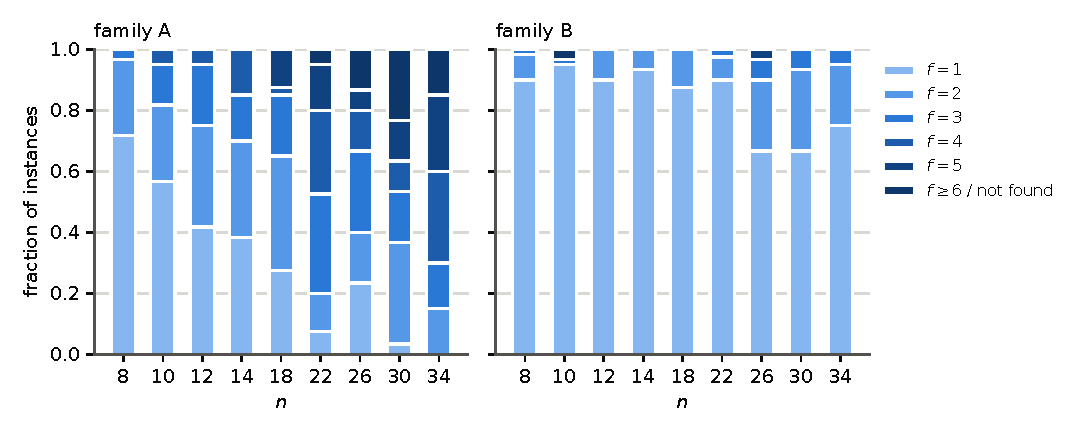
\includegraphics[width=\linewidth]{../figures/fig_fragility_distribution.pdf}
\caption{Distribution of the exact signed fragility number for \textsc{any} (rule C) as a function of $n$, families A and B, from E2 ($n\le14$) and E4 ($n\ge18$; search capped at $|R|\le\EfourKmax$, the top segment collects $f\ge6$ and not found).}
\label{fig:dist}
\end{figure}

\begin{figure}[t]
\centering
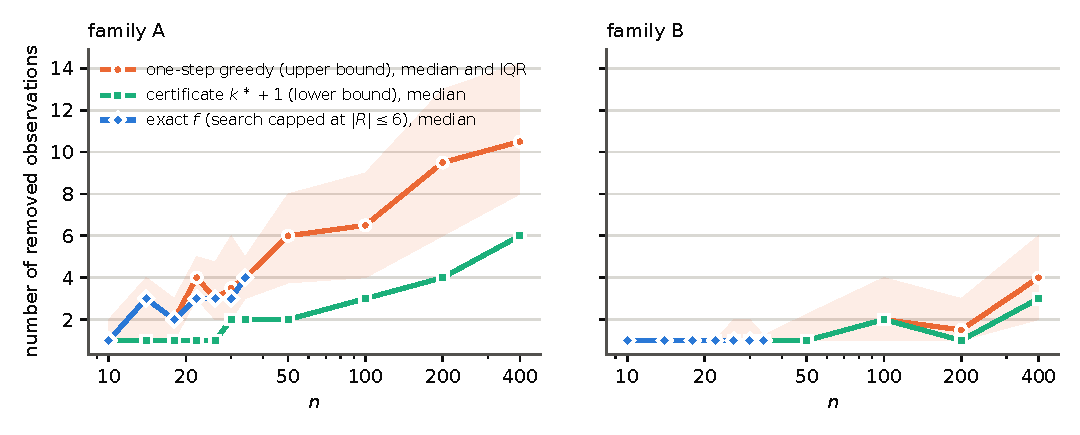
\includegraphics[width=\linewidth]{../figures/fig_bracket.pdf}
\caption{Bracketing the fragility number at large $n$ (rule C): median one-step greedy witness size (upper bound, with interquartile range) and median certified lower bound $k^\ast+1$ from Proposition~\ref{prop:cert}, per family; exact medians from E4 where available.}
\label{fig:bracket}
\end{figure}

\subsection{E5: frequency of non-monotone pairs}
For every instance of E2 with a finite targeted fragility number, all one-element supersets $R\cup\{i\}$ of up to 20 minimal witnesses $R$ were refitted. For \textsc{leave} of the weakest variable, the variable had re-entered the support in \EfiveALeaveFracPairs\% of the \EfiveALeavePairs{} superset pairs of family A (at least one re-entry in \EfiveALeaveFracInst\% of the \EfiveALeaveInstances{} instances) and in \EfiveBLeaveFracPairs\% of \EfiveBLeavePairs{} pairs of family B (\EfiveBLeaveFracInst\% of \EfiveBLeaveInstances{} instances). For \textsc{any}, the original support was restored by adding one observation to a minimal witness in \EfiveAAnyFracPairs\% (A) and \EfiveBAnyFracPairs\% (B) of the pairs (Table~\ref{tab:e5}). Non-monotonicity is thus not a curiosity of constructed examples but a regular feature of minimal witnesses on these designs.

\begin{table}[t]
\centering\small
\begin{tabular}{llrrrrrr}
\toprule
fam. & $n$ & \textsc{leave}: instances & re-entry (instances) & re-entry (pairs) & \textsc{any}: instances & restored (instances) & restored (pairs)\\
\midrule
A & 8 & 60 & 48\% & 8.9\% & 60 & 60\% & 8.9\% \\
A & 10 & 60 & 48\% & 6.6\% & 60 & 73\% & 10.5\% \\
A & 12 & 59 & 49\% & 4.9\% & 60 & 82\% & 18.3\% \\
A & 14 & 49 & 59\% & 8.4\% & 60 & 83\% & 17.3\% \\
B & 8 & 60 & 62\% & 8.4\% & 60 & 55\% & 6.9\% \\
B & 10 & 57 & 75\% & 10.3\% & 58 & 72\% & 7.6\% \\
B & 12 & 58 & 74\% & 8.9\% & 60 & 83\% & 10.5\% \\
B & 14 & 57 & 77\% & 12.3\% & 60 & 77\% & 10.5\% \\
\\
\bottomrule
\end{tabular}
\caption{E5. One-element supersets of minimal witnesses (rule C): fraction of instances with at least one non-monotone pair and fraction of superset pairs that are non-monotone.}
\label{tab:e5}
\end{table}

\section{What can be claimed}\label{sec:claims}

\begin{table}[h]
\centering\small
\begin{tabular}{p{0.70\linewidth}l}
\toprule
claim & status\\
\midrule
Unique Lasso minimiser has $X_S$ of full column rank; uniqueness under full rank of $X_E$ (Lemma~\ref{lem:rank}) & literature\\
Exact closed-form test of whether removing $R$ preserves the signed support, both rules (Prop.~\ref{prop:exact}) & proved here\\
\quad agreement with refits in \EoneSingleAgree/\EoneSingleTests{} single and \EoneMultiAgree/\EoneMultiTests{} multiple removals (E1) & verified\\
Single removal reduces to a DFBETA-type formula with the Lasso residual; $O(np)$ certificate for $f\ge2$ (Cor.~\ref{cor:single}) & proved here\\
Polynomial certificate for $f\ge k+1$ (Prop.~\ref{prop:cert}) & proved here\\
\quad certifies $k^\ast\ge1$ in \EtwoAKstarGeOne\% of family-A instances with $f\ge2$, $n\le14$; loose (E1, E2, E4) & verified\\
Witness families are not monotone: hand-checkable example with $p=1$ (Ex.~\ref{ex:one}) & proved here\\
Competition example with $p=2$, exact rational KKT certificate (Ex.~\ref{ex:two}) & verified (exact arithmetic)\\
$f_{\textsc{leave}(j)}>\lceil n/2\rceil$ implies stability-selection frequency $1$; converse not implied (Rem.~\ref{rem:stabsel}) & proved here\\
Existence of a deselection witness is NP-complete for $p=1$; fragility number NP-hard in general (Thm.~\ref{thm:hard}a) & proved here\\
Selection witnesses for $p=1$ in $O(n\log n)$ (Thm.~\ref{thm:hard}b) & proved here\\
NP-completeness of selection witnesses for $p\ge2$ (Conj.~\ref{conj:enter}) & conjectural\\
Single-removal fragility ($f=1$) in \EtwoBFracOne\% (B) and \EtwoAFracOne\% (A) of instances with $n\le14$; minimal witnesses mostly single events (E2) & verified, these designs only\\
No heuristic meets the predefined advantage criterion at $n\le14$; one-step greedy most accurate, cheap only for $n\ge22$ (E3, E4) & verified, these designs only\\
Non-monotone pairs among one-element supersets of minimal witnesses in a measurable fraction of cases (E5) & verified, these designs only\\
Rates of $f/n$ with $n$; behaviour on real data; novelty of the algebra & not claimed\\
\bottomrule
\end{tabular}
\caption{Claims and their status. ``Verified'' means reproduced by the scripts of Appendix~\ref{app:repro} with the fixed seeds; it is not a proof and it is specific to the two synthetic families.}
\label{tab:claims}
\end{table}

\paragraph{Limitations.} The exact test presupposes a unique minimiser and full column rank on the support; ties are measure-zero for continuous designs but real in integer data, and the code counts them rather than resolving them. The certificate of Proposition~\ref{prop:cert} is loose and restricted to $k<n/s_0$. The hardness statement is for $p=1$ and is weak in the technical sense; it says nothing about the difficulty of typical instances, on which exhaustive search with the closed-form test was fast. The experiments use two synthetic families, one solver, and a cap on the size of removal sets; the fragility numbers reported are exact under that cap and are not estimates of anything beyond the families. The comparison with heuristics is on a single machine and the cost ratios depend on the implementation (a vectorised test against a Python-level loop of refits).

\paragraph{Next steps for the research line.} (a) Prove or refute Conjecture~\ref{conj:enter}, and settle the complexity of \textsc{leave} for fixed $p\ge2$ in the strong sense (the $p=1$ argument only gives weak hardness). (b) Tighten Proposition~\ref{prop:cert} by exploiting the sign structure of the interaction term or by a small semidefinite relaxation, and measure the gap to $f$ on E4. (c) Replace the fixed-$\mu$ setting by a data-driven rule (cross-validation), for which the witness must account for the change of $\mu$ itself. (d) Extend the exact test to the elastic net and to the square-root Lasso, whose KKT systems are also linear on a fixed signed support.

\appendix
\section{Reproducibility}\label{app:repro}
{\sloppy The directory contains \path{experiments/lasso_fragility.py} (library: solver wrappers, Proposition~\ref{prop:exact} vectorised over subsets, Corollary~\ref{cor:single}, Proposition~\ref{prop:cert}, exhaustive search, the three heuristics, instance generator), \path{experiments/exact_examples.py} (E0), \path{experiments/run_validation.py} (E1), \path{experiments/run_fragility.py} (E2, E3, E5), \path{experiments/run_scaling.py} (E4), \path{experiments/make_figures.py} and \path{experiments/make_numbers.py}, which converts \path{results/*.json} into the macros and table bodies of this document, so that no number in the text is typed. The run scripts accept \texttt{--fast}. The reference run used Python \MetaPython, NumPy \MetaNumpy, SciPy \MetaScipy, scikit-learn \MetaSklearn~\citep{pedregosa2011}, seeds \MetaSeed{} and \MetaSeedScaling, and took \MetaSecondsValidation~s (E1), \MetaSecondsFragility~s (E2/E3/E5) and \MetaSecondsScaling~s (E4) on one core of a shared four-core machine, \MetaMinutesTotal~minutes in all.\par}

\paragraph{Solver.} \texttt{lars\_path(X, y, method="lasso", alpha\_min=$\mu/n'$)} on the reduced data with $n'$ rows; the last column of the path is the minimiser of \eqref{eq:lasso} at penalty $\mu$. Supports are read off exact zeros of the homotopy output (threshold $10^{-10}$).
\paragraph{Exact test.} For a batch of subsets of equal size $k$: $H_R$ by one batched matrix product, $e_R$ by a batched solve, $\det(I-H_R)\le10^{-12}$ treated as rank deficient (a change), conditions (i)--(ii) of Proposition~\ref{prop:exact} with strict inequalities.
\paragraph{Exhaustive search.} Sizes $k=1,2,\dots$ in order; for the signed \textsc{any} target no refit is needed; for the other targets flagged subsets are refitted and the target read from the new support; all minimal witnesses of the minimal size (up to 50) are collected.
\paragraph{Heuristics.} One-step greedy: score $=$ normalised remaining margin (for \textsc{any}) or the target coefficient/correlation after the candidate removal, computed by Corollary~\ref{cor:single} on the current fit; budget $n-2$ removals. Sorted scores: one scoring pass on the full data per direction (each active coefficient towards zero; each inactive correlation towards $+\mu$ and $-\mu$), $k_{\mathrm{pred}}$ from the cumulative sums, direction with the smallest $k_{\mathrm{pred}}$, then refits along the fixed order from $k=1$. Cook: largest $h_ie_i^2$ on the current active-set regression.
\paragraph{Exact arithmetic.} Example~\ref{ex:two}: the KKT system on the candidate support is solved with Python \texttt{fractions}, signs and inactive inequalities are checked strictly, and the stability-selection frequency is computed by enumerating all $\binom{5}{2}$ subsamples.

\bibliographystyle{plainnat}
\bibliography{refs}
\end{document}
